\begin{exercice*}
    \begin{enumerate}
        \item Construire $C$, l'image de $B$ par la rotation de centre $A$ et d'angle \ang{90}.\\
        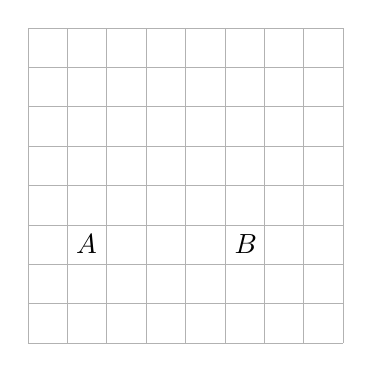
\begin{tikzpicture}[scale = 0.5]
            \draw[help lines, color=black!30] (0,0) grid (8,8);        
            \coordinate[label=below left:$A$] (A) at (2,3);
            \coordinate[label=below right:$B$] (B) at (5,3);
            \tkzDrawPoints[shape=cross out,size=3pt](A,B);
        \end{tikzpicture}
        \item Construire $F$, l'image de $E$ par la rotation de centre $D$ et d'angle \ang{90}.\\
        \begin{tikzpicture}[scale = 0.5]
            \foreach \x in {0,1,...,8} {
                \foreach \y in {0,1,...,8} {
                    \fill[color=black] (\x,\y) circle (0.05);
                }
            }
            \coordinate[label=above left:$E$] (E) at (3,7);
            \coordinate[label=above right:$F$] (F) at (5,4);
            \tkzDrawPoints[shape=cross out,size=3pt](E,F);
        \end{tikzpicture}
        \item Construire $K$, l'image de $H$ par la rotation de centre $G$ et d'angle \ang{60}.\\
        \begin{tikzpicture}[scale=0.5]
            \foreach \x in {0,...,7} {
                \foreach \y in {0,1.73,...,6.92} {
                    \fill (\x,\y) circle (0.05);
                }
            }       
            \foreach \x in {0.5,1.5,...,7.5} {
                \foreach \y in {0.865,2.595,...,7.785} {
                    \fill (\x,\y) circle (0.05);
                }
            }      
            \coordinate[label=above left:$H$] (H) at (4.5,6.055);
            \coordinate[label=above right:$G$] (G) at (6,3.46);
            \tkzDrawPoints[shape=cross out,size=3pt](H,G);
        \end{tikzpicture}
        \item Construire $N$, l'image de $M$ par la rotation de centre $L$ et d'angle \ang{120}.\\
        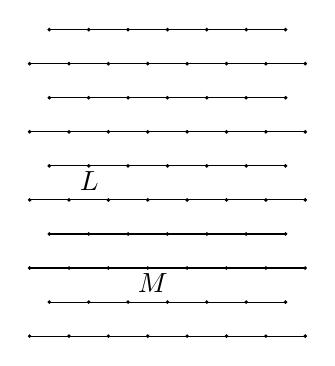
\begin{tikzpicture}[scale=0.5]
            \foreach \x in {0,...,7} {
                \foreach \y in {0,1.73,...,6.92} {
                    \fill (\x,\y) circle (0.05);
                    \draw (0,\y)--(7,\y);
                }
            }       
            \foreach \x in {0.5,1.5,...,6.5} {
                \foreach \y in {0.865,2.595,...,7.785} {
                    \fill (\x,\y) circle (0.05);
                    \draw (0.5,\y)--(6.5,\y);
                }
            }      
            \coordinate[label=above left:$L$] (L) at (2,3.46);
            \coordinate[label=above right:$M$] (M) at (2.5,0.865);
            \tkzDrawPoints[shape=cross out,size=3pt](L,M);
        \end{tikzpicture}
        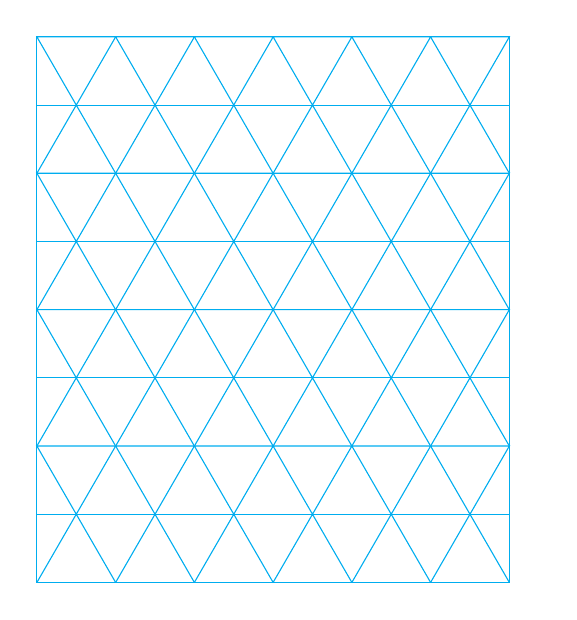
\begin{tikzpicture}
        
            \def\nx{5}
            \def\ny{3} \pgfmathsetmacro\nyy{(2+2*\ny)*sin(60)}
            
            \draw[cyan] (0,0) rectangle (\nx +1,\nyy);
            \foreach \j in {0,...,\ny} {
                \foreach \i in {0,...,\nx} {
                    \draw[cyan](0:\i)++(90:{(1+2*\j)*sin(60)})--++(1,0);
                    \draw[cyan](0:\i) ++(60:\j) ++(120:\j) node {} --++(60:2) node {} --++(-1,0) node {} --++(-60:1) node {} --++(-60:1) node {};
                }
            }
        \end{tikzpicture}
    \end{enumerate}
\end{exercice*}
\begin{corrige}
    %\setcounter{partie}{0} % Pour s'assurer que le compteur de \partie est à zéro dans les corrigés
    % \phantom{rrr}    
    \dots
\end{corrige}

